\documentclass[14pt, fleqn, xcolor={dvipsnames, table}]{beamer}
\usepackage[T2A]{fontenc}
\usepackage[utf8]{inputenc}
\usepackage[english,russian]{babel}
\usepackage{amssymb,amsfonts,amsmath,mathtext}
\usepackage{cite,enumerate,float,indentfirst}
\usepackage{cancel}
\usepackage{graphicx}
\usepackage{animate}
\usepackage{ulem}

\usepackage{tikz}
% \usepackage{enumitem}
\usetikzlibrary{shadows}

% \usepackage{enumitem}
% \setitemize{label=\usebeamerfont*{itemize item}%
%   \usebeamercolor[fg]{itemize item}
%   \usebeamertemplate{itemize item}}

\graphicspath{{images/}}

\usetheme{Madrid}
\usecolortheme{seahorse}
\renewcommand{\CancelColor}{\color{red}}

\setbeamercolor{footline}{fg=Blue!50}
\setbeamertemplate{footline}{
  \leavevmode%
  \hbox{%
  \begin{beamercolorbox}[wd=.333333\paperwidth,ht=2.25ex,dp=1ex,center]{}%
    И. Кураленок, Н. Поваров, Яндекс
  \end{beamercolorbox}%
  \begin{beamercolorbox}[wd=.333333\paperwidth,ht=2.25ex,dp=1ex,center]{}%
    Санкт-Петербург, 2014
  \end{beamercolorbox}%
  \begin{beamercolorbox}[wd=.333333\paperwidth,ht=2.25ex,dp=1ex,right]{}%
  Стр. \insertframenumber{} из \inserttotalframenumber \hspace*{2ex}
  \end{beamercolorbox}}%
  \vskip0pt%
}
\newcommand\indentdisplays[1]{%
     \everydisplay{\addtolength\displayindent{#1}%
     \addtolength\displaywidth{-#1}}}
\newcommand{\itemi}{\item[\checkmark]}

\newenvironment{mydescription}[1]
  {\begin{list}{}%  
   {\renewcommand\makelabel[1]{\color{blue}##1:\hfill}%
   \settowidth\labelwidth{\makelabel{#1}}%
   \setlength\leftmargin{\labelwidth}
   \addtolength\leftmargin{\labelsep}}}
  {\end{list}}

\title{Деревья решений\\\small{}}
\author[]{\small{%
И.~Куралёнок,
Н.~Поваров}}
\date{}
\begin{document}

\begin{frame}
\maketitle
\small
\begin{center}
\vspace{-60pt}
\normalsize {\color{red}Я}ндекс \\
\vspace{80pt}
\footnotesize СПб, 2014
\end{center}
\end{frame}

\section{Определение и пример}
\begin{frame}{Пример}
Дмитрий и Владимир выбирают страну, куда поехать на отдых. Их рассуждения:
\begin{itemize}
  \item в Америку --- далеко и много-много диких обезьян;
  \item в Европу --- дорого;
  \item в мусульманские страны не поедем: там пить нельзя;
  \item поедем в Крым!
\end{itemize}
\end{frame}

\begin{frame}{Пример}
По сути герои использовали дерево решений. Вот какими свойствами этот способ обладает:
\begin{enumerate}
  \item Легко интерпретировать (хотя тяжело понять :))
  \item Стремление к однородности групп получившихся в результате деления
  \item Деление всего множества
  \item Жадность
\end{enumerate}
\end{frame}

\begin{frame}{Свойства}
\begin{center}
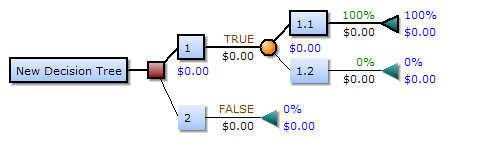
\includegraphics[width=0.9\textwidth]{Decision-Tree-Elements.png}
\end{center}
\small
\begin{itemize}
  \item Кусочно-постоянная природа
  \item Большая изменчивость при изменении learn
  \item Операции:
  \begin{itemize}
    \item Любое дерево можно представить как бинарное
    \item Дерево деревьев --- дерево
    \item Линейная комбинация, произведение, степень, etc. деревьев --- дерево
  \end{itemize}
\end{itemize}
\end{frame}

\begin{frame}{Виды деревьев}{}
\begin{itemize}
  \item Дикие
  \uncover<2->{\item Пеньки}
  \uncover<3->{\item Забывчивые}
  \uncover<4->{\item Нечеткие}
\end{itemize}
\begin{center}
\only<1>{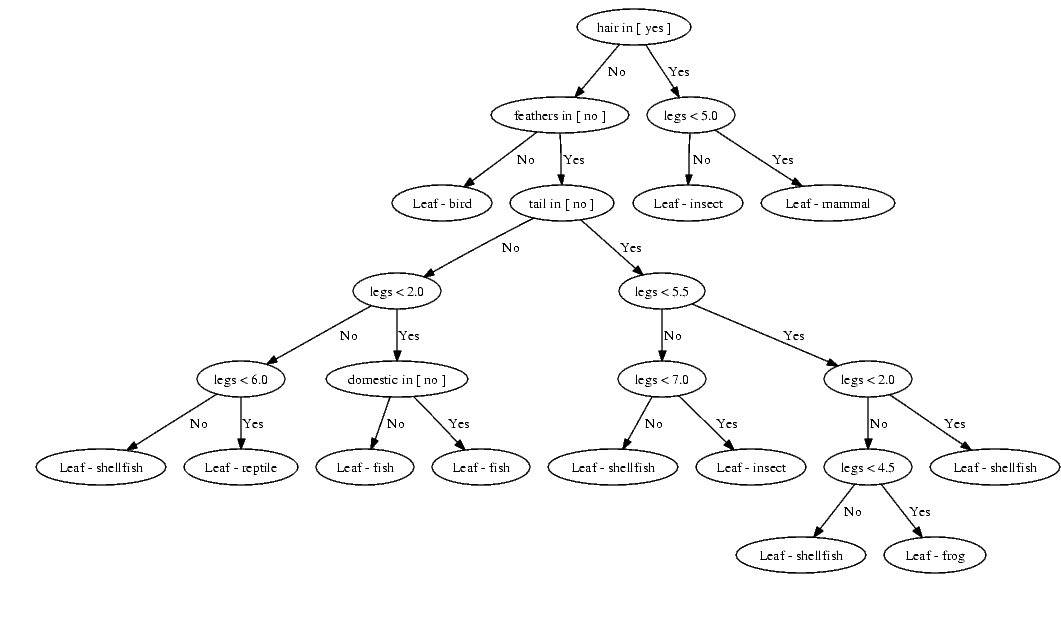
\includegraphics[height=0.4\textheight]{zooDT.png}}
\only<2>{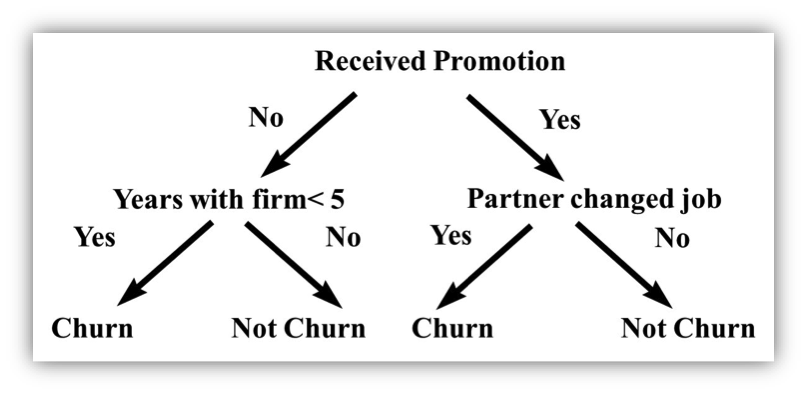
\includegraphics[height=0.4\textheight]{Decision-tree-stub.png}}
\only<3>{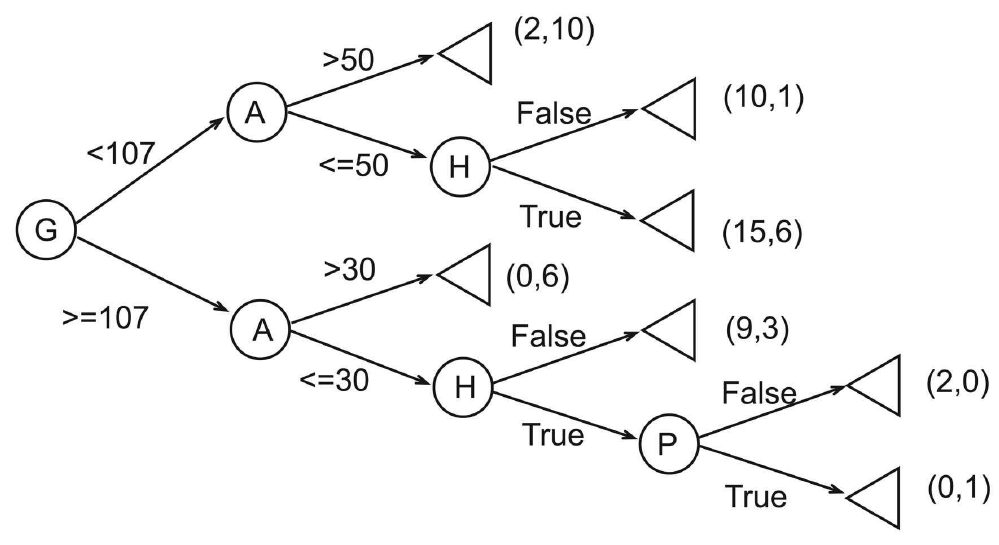
\includegraphics[height=0.4\textheight]{ObliviousTree.png}}
\only<4>{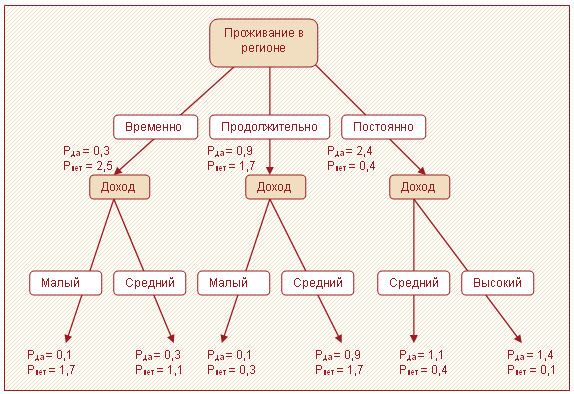
\includegraphics[height=0.4\textheight]{example_of_fuzzy_decision_tree.png}}
\end{center}
\end{frame}

\begin{frame}{Алгоритм обучения}
\small
Выберем вид обучаемого дерева, чувство прекрасного $T$, пространство точек $X$, критерий остановки $E$, правило создания листа $L$
\begin{enumerate}
  \item Вычислим изменение $T$ для всех возможных способов поделить каждый лист используя факторы из $X$
  \item Выберем максимальное улучшение $T$, проведем деление, создав листья по количеству возможных значений фактора
  \item Проверим критерий остановки $E$, если он не выполнен, идем в 1 иначе все.
  \item Подрежем дерево $P$
\end{enumerate}
По сути все обучение задается набором $T$, $X$ и $E$, $L$.
\end{frame}

\section{Алгоритмы от Quinlan}

\begin{frame}{ID3}{Iterative dichotomizer 3 (Ross Quinlan)}
\small
Строим классификатор. Алгоритм:\\
{\color{blue}$T$:} $T(l) = H(l|X) = -\sum_{x\in X} p(l(x)) p(x|l(x)) \log p(x|l(x))$\\
{\color{blue}$X$:} дискретные фичи \\
{\color{blue}$E$:} пока в листе не окажется либо $\emptyset$, либо все значения будут в одном классе \\
{\color{blue}$L$:} создаем листья по количеству возможных значений фактора, если множество пустое, то используем значение, которое чаще всего встречается у примеров с таким значением фактора во всем множестве \\
{\color{blue}$P$:} Нет
\end{frame}

\begin{frame}{C4.5}{Ross Quinlan}
\small
Строим классификатор. Алгоритм:\\
{\color{blue}$T$:} $T(l) = H(l|X) = -\sum_{x\in X} p(l(x)) p(x|l(x)) \log p(x|l(x))$\\
{\color{blue}$X$:} дискретные и непрерывные фичи, веса точек, не все точки размечены \\
{\color{blue}$E$:} пока в листе не окажется либо $\emptyset$, либо все значения будут в одном классе \\
{\color{blue}$L$:} создаем листья по количеству возможных значений фактора (в случае непрерывной фичи используем разницу не менее $\alpha$), если множество пустое, то используем значение, которое чаще всего встречается на предыдущем уровне\\
{\color{blue}$P$:} По CV сворачиваем ветви, которые не работают
\end{frame}

\begin{frame}{C5}{Ross Quinlan}
\small
Строим классификатор. Алгоритм закрыт. Но говорят:\\
\begin{itemize}
  \item Работает быстрее и потребляет меньше памяти
  \item Строит деревья меньшей высоты
  \item Умеет работать с весами точек
  \item Поддерживает бустинг (что бы это не значило)
  \item \sout{думает за вас}.
\end{itemize}
\end{frame}

\section{Алгоритм CART}

\begin{frame}{CART I}{Classification and Regression Tree (L. Breiman, J. Friedman, et.al.)}
\small
Строим классификатор или регрессию. Дерево бинарное. Алгоритм:\\
{\color{blue}$T$:} \footnotesize $T(l)$ \\\small
{\color{blue}$X$:} все возможные разбиения по каждому фактору \\
{\color{blue}$E$:} пока можно найти разбиение $l_{t+1}: T(l_t) > T(l_{t+1})$\\
{\color{blue}$L$:} создаем 2 листа с средневыборочным значением в каждом \\
{\color{blue}$P$:} нет
\end{frame}

\begin{frame}{CART II}{Classification and Regression Tree (L. Breiman, J. Friedman, et.al.)}
Чувства прекрасного для CART:
\begin{itemize}
  \item В случае классификации, применяем impurity index:
  \begin{itemize}
    \item $T(L) = Gini(L) = \sum_l \sum_c p(y_i = c | i \in l)(1 - p(y_i=c|i \in l) = \sum_l (1 - \sum_c p(y_i=c|i \in l)^2)$
    \item $T(L) = H(L|X) = -\sum_{x\in X} p(l(x)) p(x|l(x)) \log p(x|l(x))$
    \item $T(L) = \frac{1}{|L|} \sum_{l\in L} \sum_{i \in l} I(y_i \ne y_l)$
  \end{itemize}
  \item В случае регрессии:
  $$
  T(L) = \sum_{l\in L} D_l
  $$
\end{itemize}
\end{frame}

\section{Почему это может работать}
\begin{frame}{Тонкости}
На практике мы используем варианты CART, поэтому дальше только о нем.
\begin{itemize}
  \item Одинаковые по форме деревья решений могут нести существенно разную информацию
  \item Уверенность в значении в листе не всегда можно просто вычислить
  \item Не всегда оптимально назначать средневыборочное как значение в листе O\_o
\end{itemize}
\end{frame}

\subsection{Количество информации в дереве}

\begin{frame}{Немного о информации}
Сколько всего информации в дереве:
\begin{itemize}
  \item Информация о способе разбиения в каждом ноде: $\log(n) + \log(|f_l|)$
  \item Информация о получившемся разбиении: $\sum_{l \in L} \frac{|l|}{|X|} \log (|l|)$
  \item Значения в листьях: $|L|\times32bit$
\end{itemize}
$\Rightarrow$ Круто оптимизировать разбиения фичи \\
$\Rightarrow$ Мы можем построить prior по тому, сколько в дереве информации (сага о $\log$)
\end{frame}

\begin{frame}{Способы бинаризации}
\small
$$
X \subset \mathbb{R}^{n\times m}, b: \mathbb{R}^n \to \{0,1\}^N
$$
По хорошему, хотим $\hat{b} = \arg_b \max T\left(V,\arg \max_F(b) T(L,F)\right)$, но это дорого и долго, поэтому используем эмпирику, например медианное разбиение с фиксированным количеством слотов.
\end{frame}

\begin{frame}{Диалоги о дисперсии}
\small
В случае MSE минимизируем суммарную дисперсию на каждом сплите. Дисперсия растет с числом точек, нам интересно, что будет на бесконечности.
\begin{center}
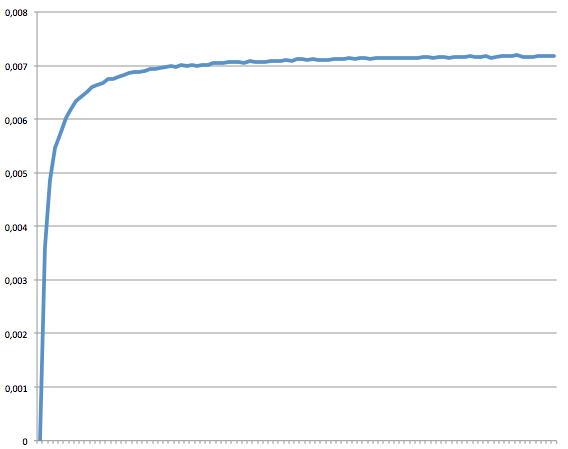
\includegraphics[height=0.5\textheight]{D.png} 
\end{center}
Можно использовать исправленную дисперсию, но помогает не всегда и есть варианты.
\end{frame}

\begin{frame}{Диалоги о ожидании I} % Stein paradox
Только что мы поняли, что среднее отклонение по выборке работает плохо. А как же быть со средним выборочным в качестве мат ожидания. \\
Проведем такой эксперимент: возьмем случайный нормальный вектор с единичной матрицей ковариаций и ненулевым, сравнимым с 1 ожиданием $\mu$. Хотим найти $\hat{\theta}: \min \|\theta - \mu\|$. В этом случае очевидное решение $\hat{\theta} = \frac{1}{n}\sum x_i$, окажется неоптимальным. % см код DispersionTest
\end{frame}

\begin{frame}{Диалоги о ожидании II} 
Нам парадокс Штайна интересен в двух аспектах:
\begin{enumerate}
  \item Вычисляя среднее в листе, мы можем считать, что у нас есть 1 реализация вектора размерности $n$ и применить магию js-поправки.
  \item Принадлежность точки к ноду можно считать подругому: $\sum_i I\{x_{f(i)} > c_i\} > l$, где $f(i)$ --- номер фактора, использованного при делении на $i$-м уровне, $c_i$ --- условие деления. Сама сумма может быть рассмотрена как сумма бернуллевских случайных величин в условиях данной точки и к ней можно попробовать применить поправку Штайна.
\end{enumerate}
\end{frame}

\begin{frame}{Диалоги о ожидании III} % Stein paradox
Все было бы хорошо, если бы:
\begin{itemize}
  \item Поправка была бы устойчива к ошибкам; % см test1FoldErr10 где js сливает наиву в одну калитку
  \item Мы хорошо бы знали дисперсию и форму распределения.
\end{itemize}
\end{frame}


% \section{Пара трюков}
% \subsection{Гистограммы}
% \subsection{Разложение целевой функции в ряд}

\begin{frame}{Что мы сегодня узнали}
\begin{itemize}
  \item Деревья решений = разделяй и влавствуй
  \item Жадность + ограничение информации в делении = Profit
  \item Есть много чувств прекрасного, и хорошее еще не изобретено
  \item Много нюансов есть в очень простых вещах, даже в вычислении среднего :)
\end{itemize}
\end{frame}
\end{document}
